\documentclass[10pt]{article}

\usepackage{amsmath}

\numberwithin{equation}{section}

\usepackage[english]{babel}
\usepackage[utf8]{inputenc}
\usepackage{amsfonts}
\usepackage{graphicx}
\usepackage{epstopdf}
\usepackage{caption}
\usepackage{float}
\usepackage{bm}
\usepackage{esvect}
\usepackage{hyperref}
\usepackage{listings}

\usepackage{setspace}
\onehalfspacing

\oddsidemargin = -5pt
\evensidemargin = -5pt
\textwidth = 500pt
\topmargin = -50pt
\textheight = 650pt

\title{SPM Report}
\date{}
\author{
	Massimo Equi\\
	AY 2017/2018
}

\begin{document}
\maketitle

\section{Introduction}  \label{intro}
The chosen project is the one consisting in using a genetic algorithm to estimate an unknown function $f$ given a set of pairs $\left(x, f\left(x\right)\right)$ as input.

\section{User Manual} \label{usermanual}
In order to compile and run the program follow these instructions:
\begin{itemize}
\item move to the \verb|SPM_FinalProject| directory;
\item if needed, run the command \verb|make clean|, it will remove all the \verb|.o| and \verb|.out| files; 
\item compile the program with the command \verb|make -f [makefile]|
\item run the sequential program with \verb|./main.out [parameters] < [input_file]|
\item run the parallel program with \verb|./parallel_main.out [parameters] < [input_file]|
Here it is an example of a typical session:
\begin{verbatim}
$ make clean
$ make -f Makefile.icc
$ make -f Makefile.ff.icc
$ make -f Makefile.thread.icc
$ ./main.out 12000 5 4000 10 -1 20 0.5 no < "input_cos(x)-pow(x,3)10-3.txt"
$ ./ff_main.out 12000 5 4000 10 -1 20 0.5 8 no < "input_cos(x)-pow(x,3)10-3.txt"
$ ./thread_main.out 12000 5 4000 10 -1 20 0.5 8 no < "input_cos(x)-pow(x,3)10-3.txt"
\end{verbatim}
\paragraph{Makefile}
For compiling the sequential program, \verb|[makefile]| can be one of the following:
\begin{itemize}
	\item \verb|-f Makefile| (or simply \verb|make|) compiles the program with the \verb|g++| compiler;
	\item \verb|-f Makefile.icc| compiles the program with the \verb|icc| compiler;
	\item \verb|-f Makefile.icc.mic| compiles the program with the \verb|icc| compiler using the flag \verb|-mmic|;
\end{itemize}
All of the above commands output a \verb|main.out| file.\\
For compiling the FastFlow version of the program, \verb|[makefile]| can be one of the following:
\begin{itemize}
	\item \verb|make -f Makefile.ff| compiles the program with the \verb|g++| compiler;
	\item \verb|make -f Makefile.ff.icc| compiles the program with the \verb|icc| compiler;
	\item \verb|make -f Makefile.ff.icc.mic| compiles the program with the \verb|icc| compiler using the flag \verb|-mmic|;
\end{itemize}
All of the above commands output a \verb|ff_main.out| file.
For compiling the version of the program that uses threads, \verb|[makefile]| can be one of the following:
\begin{itemize}
	\item \verb|make -f Makefile.thread| compiles the program with the \verb|g++| compiler;
	\item \verb|make -f Makefile.thread.icc| compiles the program with the \verb|icc| compiler;
	\item \verb|make -f Makefile.thread.icc.mic| compiles the program with the \verb|icc| compiler using the flag \verb|-mmic|;
\end{itemize}
All of the above commands output a \verb|thread_main.out| file.
\paragraph{Run the program}
The program runs with several parameters and has to be called with an input file. Calling \verb|./main.out|, \verb|./ff_main.out| or \verb|./thread_main.out| with no arguments will show a quick guide. \verb|[parameters]| consists in the following: 
\begin{itemize}
	\item \verb|tree_no| is the number of trees that will be created in the random pool generated at the beginning of every execution;
	\item \verb|depthmax| is the maximum possible depth a tree in the pool can have;
	\item \verb|threshold| is the number of trees the algorithm will select to generate the next population (has to be lesser than \verb|tree_no|);
	\item \verb|randmax| is the largest value a leaf of a tree holding a constant can have;
	\item \verb|randseed| is the seed used for \verb|std::srand()|. If \verb|randseed| is a negative number \verb|std::time(nullptr)| is used as seed;
	\item \verb|gen_no| is the number of generations such that, once reached, the algorithm will terminate;
	\item \verb|err| is the threshold for the fitness. If the fitness of the best tree is lesser that \verb|err| the program will terminate. If \verb|err| is a negative number the algorithm will stop only after reaching \verb|gen_no| generations;
	\item \verb|nw| is the number of parallel workers (skip this argument if the program is sequential);
	\item \verb|debug| can be either \verb|yes| or \verb|no|; if it is \verb|yes| it runs the program with detailed information at each generation.	   
\end{itemize}
The program requires an input file to run. Any file in this project's root directory whose name begins with the string \verb|input_| is a legal input file. In all the executions mentioned in this report we used the input file \verb|input_cos(x)-pow(x,3)10-4.txt| (\verb|10-4| in the name of the file means there are $10^4$ input pairs $(x,f(x))$ in that file).\\
After having compiled the main program, the command \verb|make [makefile] test| can be used to generate \verb|test_FitnessTime.out|. This little test program can be executed specifying an input file (and no arguments) in order to get some estimations about the time needed to evaluate a tree and compute the fitness function.
\end{itemize}

\section{Structure of the code} \label{codestructure}
The code has two main directories: \verb|src/| is where the \verb|.cpp| source files are located while \verb|include/| is where the \verb|.h| header files can be found. Both \verb|src/| and \verb|include/| are structured in three subdirectories: \verb|grammar/|, \verb|genetics/| and \verb|main/|.

\paragraph{grammar}
In \verb|grammar/| there are all the classes needed to implement the grammar provided in the project assignment. Every class is implementing a nonterminal symbol of the grammar with methods that allows it to be expanded using one of its production. The nonterminal \verb|<unop>| and \verb|<binop>| are directly encapsulated in the class \verb|Node| which of course implement the nonterminal \verb|<node>|. Each of these classes gives a concrete implementation of the abstract class \verb|INode|, which is meant to represent a generic node in the syntax tree. An object of class \verb|Node| can be randomly expanded to a given depth using the method \verb|Node::expandRandom()|. Finally, the parameter \verb|randmax| gives and upper bound to the highest number that the class \verb|Const| can store.

\paragraph{genetics}
In \verb|genetics/| the class \verb|Tree| is implementing the behavior of a syntax tree meant to represent a function. Basically, \verb|Tree| provides a nice interface to store and manage the root node of this syntax tree. The class \verb|Forest| is the core of the algorithm since it manages a pool of \verb|Tree|s providing methods to perform mutation and crossover over them. The two classes \verb|FF_Forest| and \verb|ThreadForest| are subclasses of \verb|Forest| and they are used to override the part of the code that was chosen to be turned from sequential to parallel.

\paragraph{main}
In \verb|main/| the file \verb|evolution_cyle.hpp| uses a \verb|Forest| to implement the genetic algorithm. \verb|main.cpp|, \verb|ff_main.cpp| and \verb|ff_main.cpp| call \verb|evolution_cycle.hpp| passing it respectively a \verb|Forest|, a \verb|FF_Forest| or a \verb|ThreadForest|.

\section{Parallelization Choices}
\subsection{Decomposition Strategy}
The main operations that our algorithm is performing are: \emph{selection}, \emph{mutation} and \emph{crossover}, \emph{replication}. Running the sequential version of the program we see that the completion time of \emph{selection} is several orders of magnitude larger than the one needed for \emph{replication}, \emph{mutation} and \emph{crossover}. For this reason, we focused on optimizing only the \emph{selection} phase. Moreover, try to parallelize \emph{mutation} and \emph{crossover} would lead to two major issues. First, the logic of the program would change and hence the accuracy too because parallelize \emph{crossover} means assign to each worker a portion of the array storing the best trees to avoid any synchronization delay; this would imply perform \emph{crossover} among only a portion of the best trees instead all of them. Second, since \emph{mutation} and \emph{crossover} affects only the best \verb|threashold| trees, we will work in parallel on a set of trees that is much smaller than the entire pool, leading to parallelization advantages eventually non relevant. Finally, we also decided to not parallelize the \emph{replication} part because the amount of work we would do for a single tree would be too little (just copying the tree itself) due to the fact that the trees that are more likely to be reproduced are the shallower.\\
Focusing on \emph{selection} and analyzing the structure of the problem we observe that it is embarrassingly parallel at two different level of grain. At each iteration our program has to compute the fitness function of all the trees in our pool, hence for every of those trees it is required to evaluate the function that tree is representing over all input data points. This means we could parallelize:
\begin{itemize}
	\item at a \textbf{fine grain} level, evaluating in parallel the function represented by a single tree over different data points;
	\item at a \textbf{coarse grain} level, computing in parallel the fitness function for different trees.
\end{itemize}
Therefore, the first thing we have to discuss if it is worth it to parallelize at any of this two levels of grain.
\paragraph{Single tree parallelization}
In a typical execution of the code we have to handle trees whose depth is set to be not greater that $8$. This is because most of the times the best trees tent to be the shallower ones hence it is useless to set a very high depth since the deeper trees most probably will be discarded soon. Moreover, the average depth is usually smaller than $3$; this means that on the average we perform $2^{3+1}-1=15$ floating point operations per tree, assuming a floating point operation per node. This means that the amount of time we spend evaluating a tree has roughly at most $10^{-1}\mu$$s$ order of magnitude. If we compare this with the time spent to create a thread (approximately $10\mu$$s$) we realize that even if every worker of our hypothetical parallel computation processed $100$ input points this would still be comparable with the effort needed to set up the thread for that worker, hence at least $1000$ input points per thread are needed to have a reasonable advantage. Therefore, if for instance we supposed to work with $10$ workers, we would need more that $10^{4}$ input points to get any advantage from the parallelization, and this would rarely be the case. This is clearly a scenario where we would have a very poor scalability. Thus, we conclude claiming that it is not worth it to parallelize the program relaying on such a fine grain.
\paragraph{Pool parallelization}
Considering instead the whole pool of trees the workload that would be assigned to a worker in a parallel computation is reasonably large and, more importantly, increases easily with the input size. The fitness function for a tree is computed in order of $10^{2}\mu$$s$, hence having only $10$ trees per worker is already enough to get a workload of $10^{3}\mu$$s$. Typically we work with a pool consisting of thousands of trees and this usually means that every worker will have order of $10^{2}$ trees to handle, even in situations with hundreds of parallel workers. Hence we conclude that it is worth it to parallelize at this level of grain.

\subsection{Implementation of the Parallel Part of the Code}
The difference between the sequential and the parallel version of the code resides in the classes \verb|FF_Forest| and \verb|ThreadForest|. The class \verb|FF_Forest| uses a FastFlow \verb|ParallelFor| object to manage the workers needed to compute the fitness functions in parallel. The \verb|C++| sequential \verb|for| loop present in the \verb|Forest| class is replaced by a call to the FastFlow method \verb|parallel_for()|. We could use a parallel for due to the fact that no synchronization is needed among the various iterations of the loop since computing the fitness function resembles the \emph{map} pattern. The same reasoning applies in the \verb|ThreadForest| case, where instead of a parallel for we create a thread for each one of the workers passing them the starting and ending positions of the pool at within which they have to work. We leave the main thread waiting for the termination of the others. We are aware we could use a barrier and reuse the same threads at each iteration but this would have complicated a lot the logic of the code. After the \emph{selection} phase, one thread would have had to continue the execution to perform \emph{mutation}, \emph{crossover} ans \emph{replication} while all the others would have had to wait until the beginning of the next iteration, not letting us to use the standard barrier programming pattern. We estimate that the effort needed to create a thread (order of microseconds) is reasonably negligible if compared to the amount of work that thread will do (order of milliseconds), hence we have chosen the aforementioned implementation solution.

\section{Expected Results}
In our scenario we have parallelized our code using a farm pattern whose overheads resides mostly on splitting the initial task in several subtasks and assigning them to different parallel executors. Additionally, we have to point out that in the thread case the overheads of creating the workers at each iteration could be particularly relevant when using a large amount of cores on the PHI machine. In fact, when using hundreds of cores the per thread workload could become comparable to the setup time for that thread, leading to bad scalability.\\
Another issue that could make our performances worse is a bad load balancing. Indeed, executing the sequential program, dividing the tree pool in $nw$ partitions and measuring the time spent in each of them it is possible to figure out the their workload (it can be done using \verb|make -f Makefile.test.icc| and running \verb|test_main.out| with no arguments for the quick guide). We notice that there is no particular problem with the load balancing to emphasize besides claiming that the randomization preserve it.\\
\\ 
In order to have an idea of the expected results we have run the sequential program and measured the serial and non serial fraction. Running the program with these parameters:
\begin{verbatim}
tree_no = 12000; depthmax = 5; threshold = 4000;
randmax = 10; randseed = 4; gen_no = 20; err = -1;
input file : "input_cos(x)-pow(x,3)10-4.txt"
\end{verbatim} 
We got an average completion time of $208.5606s$, with $207.9926s$ spent in the non serial part. Hence the serial fraction is just $208.5606 - 207.9926 = 0.568s$. This means that in principle we could get an extremely high speedup (order of $400$). In practice we have to take into account that such a speedup requires a very large input size to counterbalance the extreme splitting that would be made for the tree pool. Hence we expect to have a speedup mostly limited by the overheads the parallel implementation introduces, the input size and the physical limitation of the machines.\\
Since we need to have an estimation of the completion time of our program, we will use the following analytic model to express the ideal time:
\begin{equation}
T_{id}(n) = T_{serial} + \frac{T_{nonserial}}{n}
\end{equation}
There are of course overheads (like communication times) that we are not taking into account but we argue that this model is good enough to give us a reasonable lower bound for the parallel completion time.

\section{Achieved Results}
Here we report the actual \emph{completion times} we measured on the Xeon CPU E-2650 and the Xeon PHI machines for the parallel executions of the program, alongside with the graphs for the \emph{speedup}, \emph{scalability} and \emph{efficiency}, comparing these results with the sequential program's ones. The \verb|err| parameter has been always set to \verb|-1| in order to perform exactly \verb|gen_no| iterations and we always used the same \verb|randseed| for each execution in order to get more comparable results.
\paragraph{Format of the results}
The program uses \verb|std::chrono| statements in order to output the time spent to perform the computation. We stored all the results in two files in the \verb|results/| directory: the file \verb|results_testXeon.txt| for the Xeon machine and the file \verb|results_XeaonPHI.txt| for the Xeon PHI machine. Both files has a line storing the output of the \verb|uptime| command in order to record the state of the machine at the execution time. Each one of the lines storing the results of the tests starts with the string \verb|results|. The scripts \verb|test.sh| and \verb|test.phi.sh| in the main directory run all the tests from scratch (without recording them by their own), but this requires a huge amount of time and we think it will not be needed.
\paragraph{Gathering the results}
We used this parameter setting for all the execution (of course, no \verb|nw| parameter was needed for the sequential execution). For the \textbf{Xeon} we had:
\begin{verbatim}
tree_no = 12000; depthmax = 5; threshold = 4000;
randmax = 10; randseed = 4; gen_no = 20; err = -1;
nw = [1, 2, 4, 8, 16];
\end{verbatim}
while for the \textbf{Xeon PHI} we had:
\begin{verbatim}
tree_no = 2400; depthmax = 5; threshold = 800;
randmax = 10; randseed = 4; gen_no = 20; err = -1;
nw = [1, 2, 4, 8, 16, 32, 64, 128].
\end{verbatim}
We passed \verb|"input_cos(x)-pow(x,3)10-4.txt"| as input file, hence we had $10000$ input pairs $(x, f(x))$. The smaller number of trees on the Xeon PHI is due to the lower clock speed. We performed at least $5$ runs of the program for each parameter setting, we took out eventual outliers and then we computed the average of the remaining.

\subsection{Xeon}
Looking at \figurename~\ref{fig:xeoncompletiontime} we could say that the program has achieved the expected results since the completion time in both the FastFlow and the thread case approaches the ideal one. The overhead of creating the threads results to be not too relevant, since the thread implementation has slightly worse performances than the FastFlow one. As expected, \figurename~\ref{fig:xeonspeedup} shows a speedup that, even if it is increasing, seems to be approaching a maximum point way sooner than the maybe too optimistic theoretical threshold of $~400$. This should be due to the practical limitations mentioned above. The scalability graph in \figurename~\ref{fig:xeonscalability} highlights some problems our program could have. We have run it changing the number of trees and the number of input points:
\begin{verbatim}
tree_no = 12000 and 1000 input points;
tree_no = 3000 and 1000 input points;
\end{verbatim}
and we noticed that it suffered mostly because of the smaller input size. What we could conclude from this is that with fewer input points the workload for each worker is too small to properly overcome the overheads of the parallel execution. Indeed, we tried to run the sequential and the FastFlow versions of the program with these two sets of parameters compiling them with the \verb|-O0| option. The results are reported in the file \verb|results/results_noopt.txt|. The sequential and the \verb|nw = 1| cases are shown to be drastically slower then the optimized version, while for \verb|nw > 1| we still have reasonable performances, actually closer to the ideal ones. We checked eventual vectorization optimization and found that no extra loops were vectorized in the sequential program w.r.t. the parallel one. Hence we have reason to believe that the compile time optimizations are able to significantly lower down the completion time in the sequential and in the \verb|nw = 1| cases, leading to worse scalability when using smaller inputs.

\subsection{Xeon PHI}
On the Xeon PHI machine we register a different situation. Even if the completion time of both the implementations properly approaches the ideal one, we notice that the thread version starts to suffer because of the creation of all the threads. As previously mentioned, when using a very large amount of workers the partition assigned to each of them becomes to small. We can clearly see this in the speedup graph (\figurename~\ref{fig:xeonphispeedup}): the thread implementation not only has a lower speedup than the FastFlow one, it actually reaches the maximum and starts to perform worse. We conclude that the setup time needed for the threads is becoming to be comparable with actual business logic computation time. We have this claim since the FastFlow implementation, which uses a thread pool and manage a barrier, does not seem to be harmed so much by the increasing number of workers. This fact is just emphasized by the scalability and efficiency graphs, which demonstrate that in this case the thread implementation is not able to scale properly even with a large amount of input points, while the FastFlow version of the program still preserve a fairly reasonable scalability.

\begin{figure} 
	\centering
	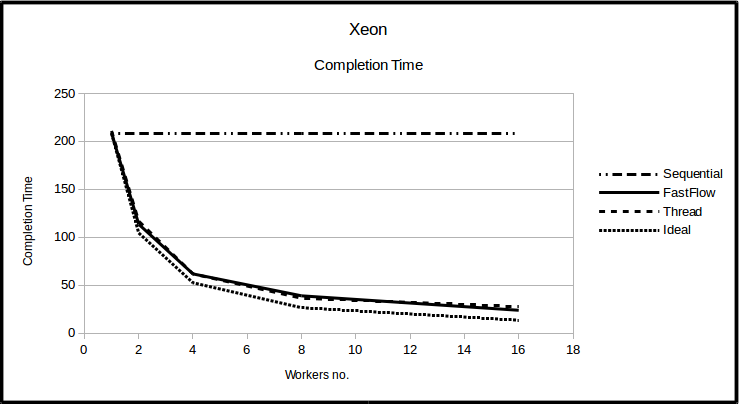
\includegraphics[scale=.5]{Xeon_CompletionTime.png}
	\caption{Completion time on the Xeon.}
	\label{fig:xeoncompletiontime}
\end{figure}

\begin{figure} 
	\centering
	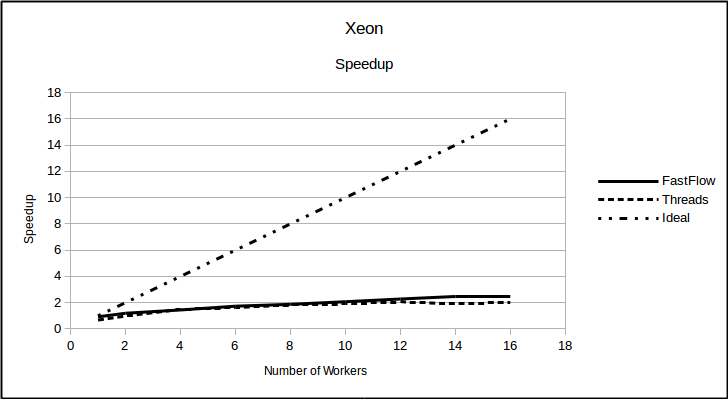
\includegraphics[scale=.5]{Xeon_Speedup.png}
	\caption{Speedup on the Xeon.}
	\label{fig:xeonspeedup}
\end{figure}

\begin{figure} 
\centering
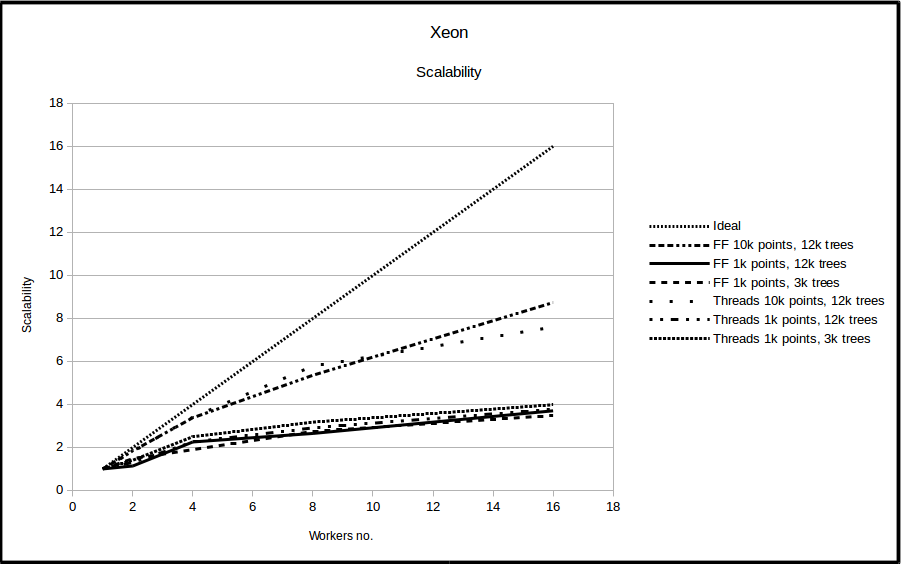
\includegraphics[scale=.75]{Xeon_Scalability.png}
\caption{Scalability on the Xeon.}
\label{fig:xeonscalability}
\end{figure}

\begin{figure} 
\centering
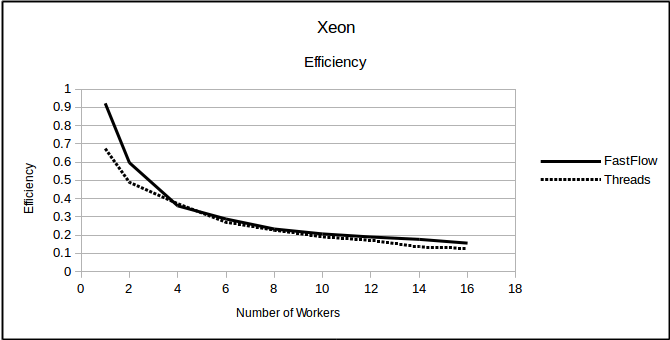
\includegraphics[scale=.5]{Xeon_Efficiency.png}
\caption{Efficiency on the Xeon.}
\label{fig:xeonefficiency}
\end{figure}

\begin{figure} 
	\centering
	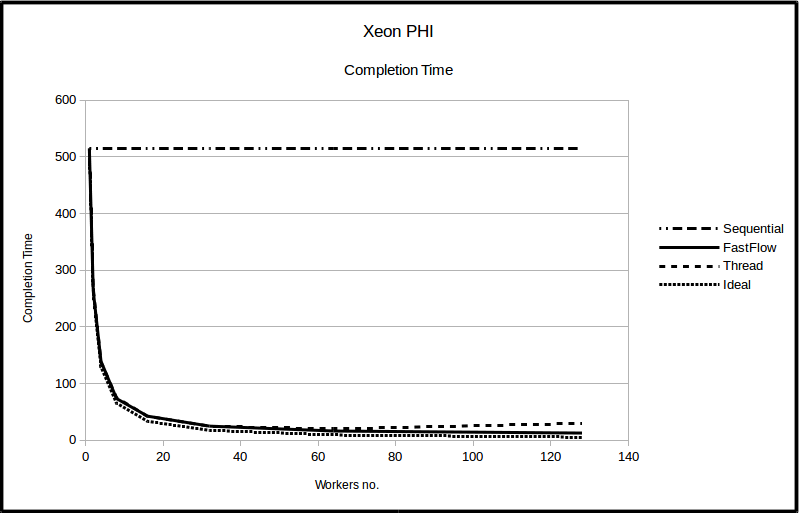
\includegraphics[scale=.5]{XeonPHI_CompletionTime.png}
	\caption{Completion time on the XeonPHI.}
	\label{fig:xeonphicompletiontime}
\end{figure}

\begin{figure} 
	\centering
	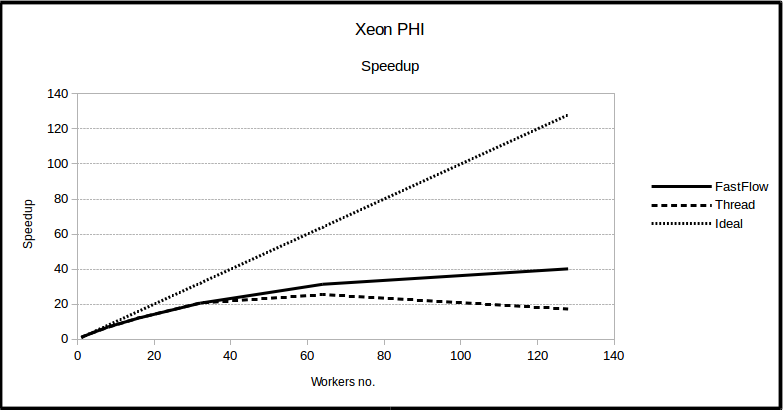
\includegraphics[scale=.5]{XeonPHI_Speedup.png}
	\caption{Speedup on the XeonPHI.}
	\label{fig:xeonphispeedup}
\end{figure}

\begin{figure} 
	\centering
	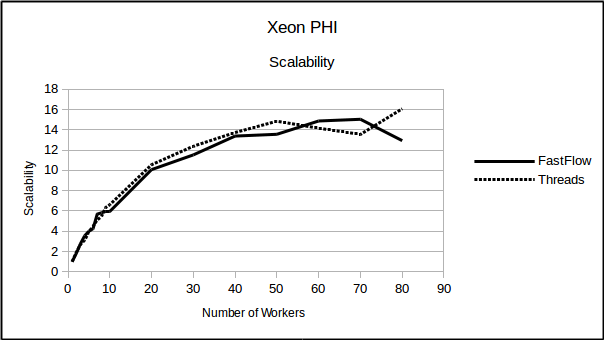
\includegraphics[scale=.75]{XeonPHI_Scalability.png}
	\caption{Scalability on the XeonPHI.}
	\label{fig:xeonphiscalability}
\end{figure}

\begin{figure} 
	\centering
	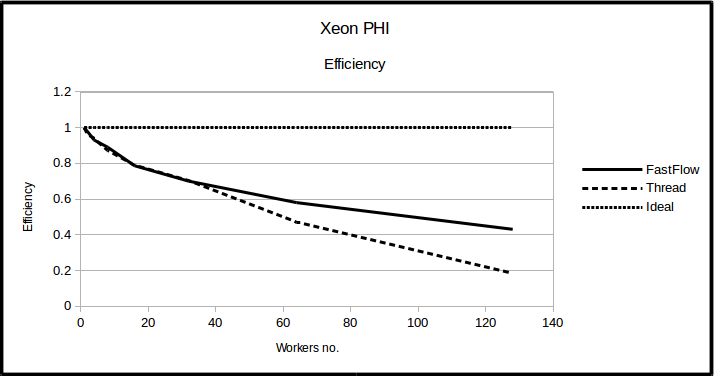
\includegraphics[scale=.5]{XeonPHI_Efficiency.png}
	\caption{Efficiency on the XeonPHI.}
	\label{fig:xeonphiefficiency}
\end{figure}

\end{document}

